\chapter{Das AUVSI Projekt}\label{cha:Das AUVSI Projekt}

Studentsiches Projekt im Labor  bla blub

\section{(Geschichte und Hintergrund) Der AUVSI Wettbewerb}

\cite{AUVSIrules}

\cite{Meiling}

-->> siehe Meiling 

\section{(Geschichte HM Team - Profs und wichtige Personen nennen) Das Studentische AUVSI Team}

-->> ggf auch Meiling

*Bilder Raussuchen

\section{(Geschichte und Hintergrund) Ecuador-Projekt}

\cite{Niclas}

\begin{figure}[H]
\centering
\includegraphics[width=0.9\textwidth]{bilder/Fotos/Ecuador_2015_Gruppenbild.jpg} 
\caption{Die Forschungsgruppe in Sharametsa} 
\label{Die Forschungsgruppe in Sharametsa}
\end{figure}


\section{(Entwicklungsgeschichte) Bisherige Flugzeuge}

Im laufe der Aktivität des UAV Projekts im Labor für Systemtechnik sind mit zunehmender Erfahrung verschiedenste Flugplattformen Betrieben worden. Die Bandbreite reicht von einfachen Modellflugzeugen bis hin zu vollständig Missionsangepassten Eigenkonstruktionen.
Dieser Abschnitt soll einen kurzen Überblick über diese Historie geben.

\begin{figure}[H]
\centering
\includegraphics[width=0.9\textwidth]{bilder/Fotos/Maya_2014.jpg} 
\caption{Erster Versuchsträger Modellflugzeug "Maja"} 
\label{Erster Versuchsträger Modellflugzeug "Maja"}
\end{figure}

Mit der eigentlich als Modellflugzeug erworbenen 'Maja' in Schaumbauweise wurden die ersten Gehversuche mit dem Ardupiloten und Telemetriesystemen im Flug unternommen. Das Knappe Platzangebot und die Moderaten Flugleistungen schränkten hier jedoch die Möglichkeiten stark ein. Auch war der Startvorgang ein nicht abzustellendes Problemfeld. Der Druckpropeller ermöglichte keinen sicheren Handstart und der Einsatz von Startwagen führte immer wieder zu Schäden.

\begin{figure}[H]
\centering
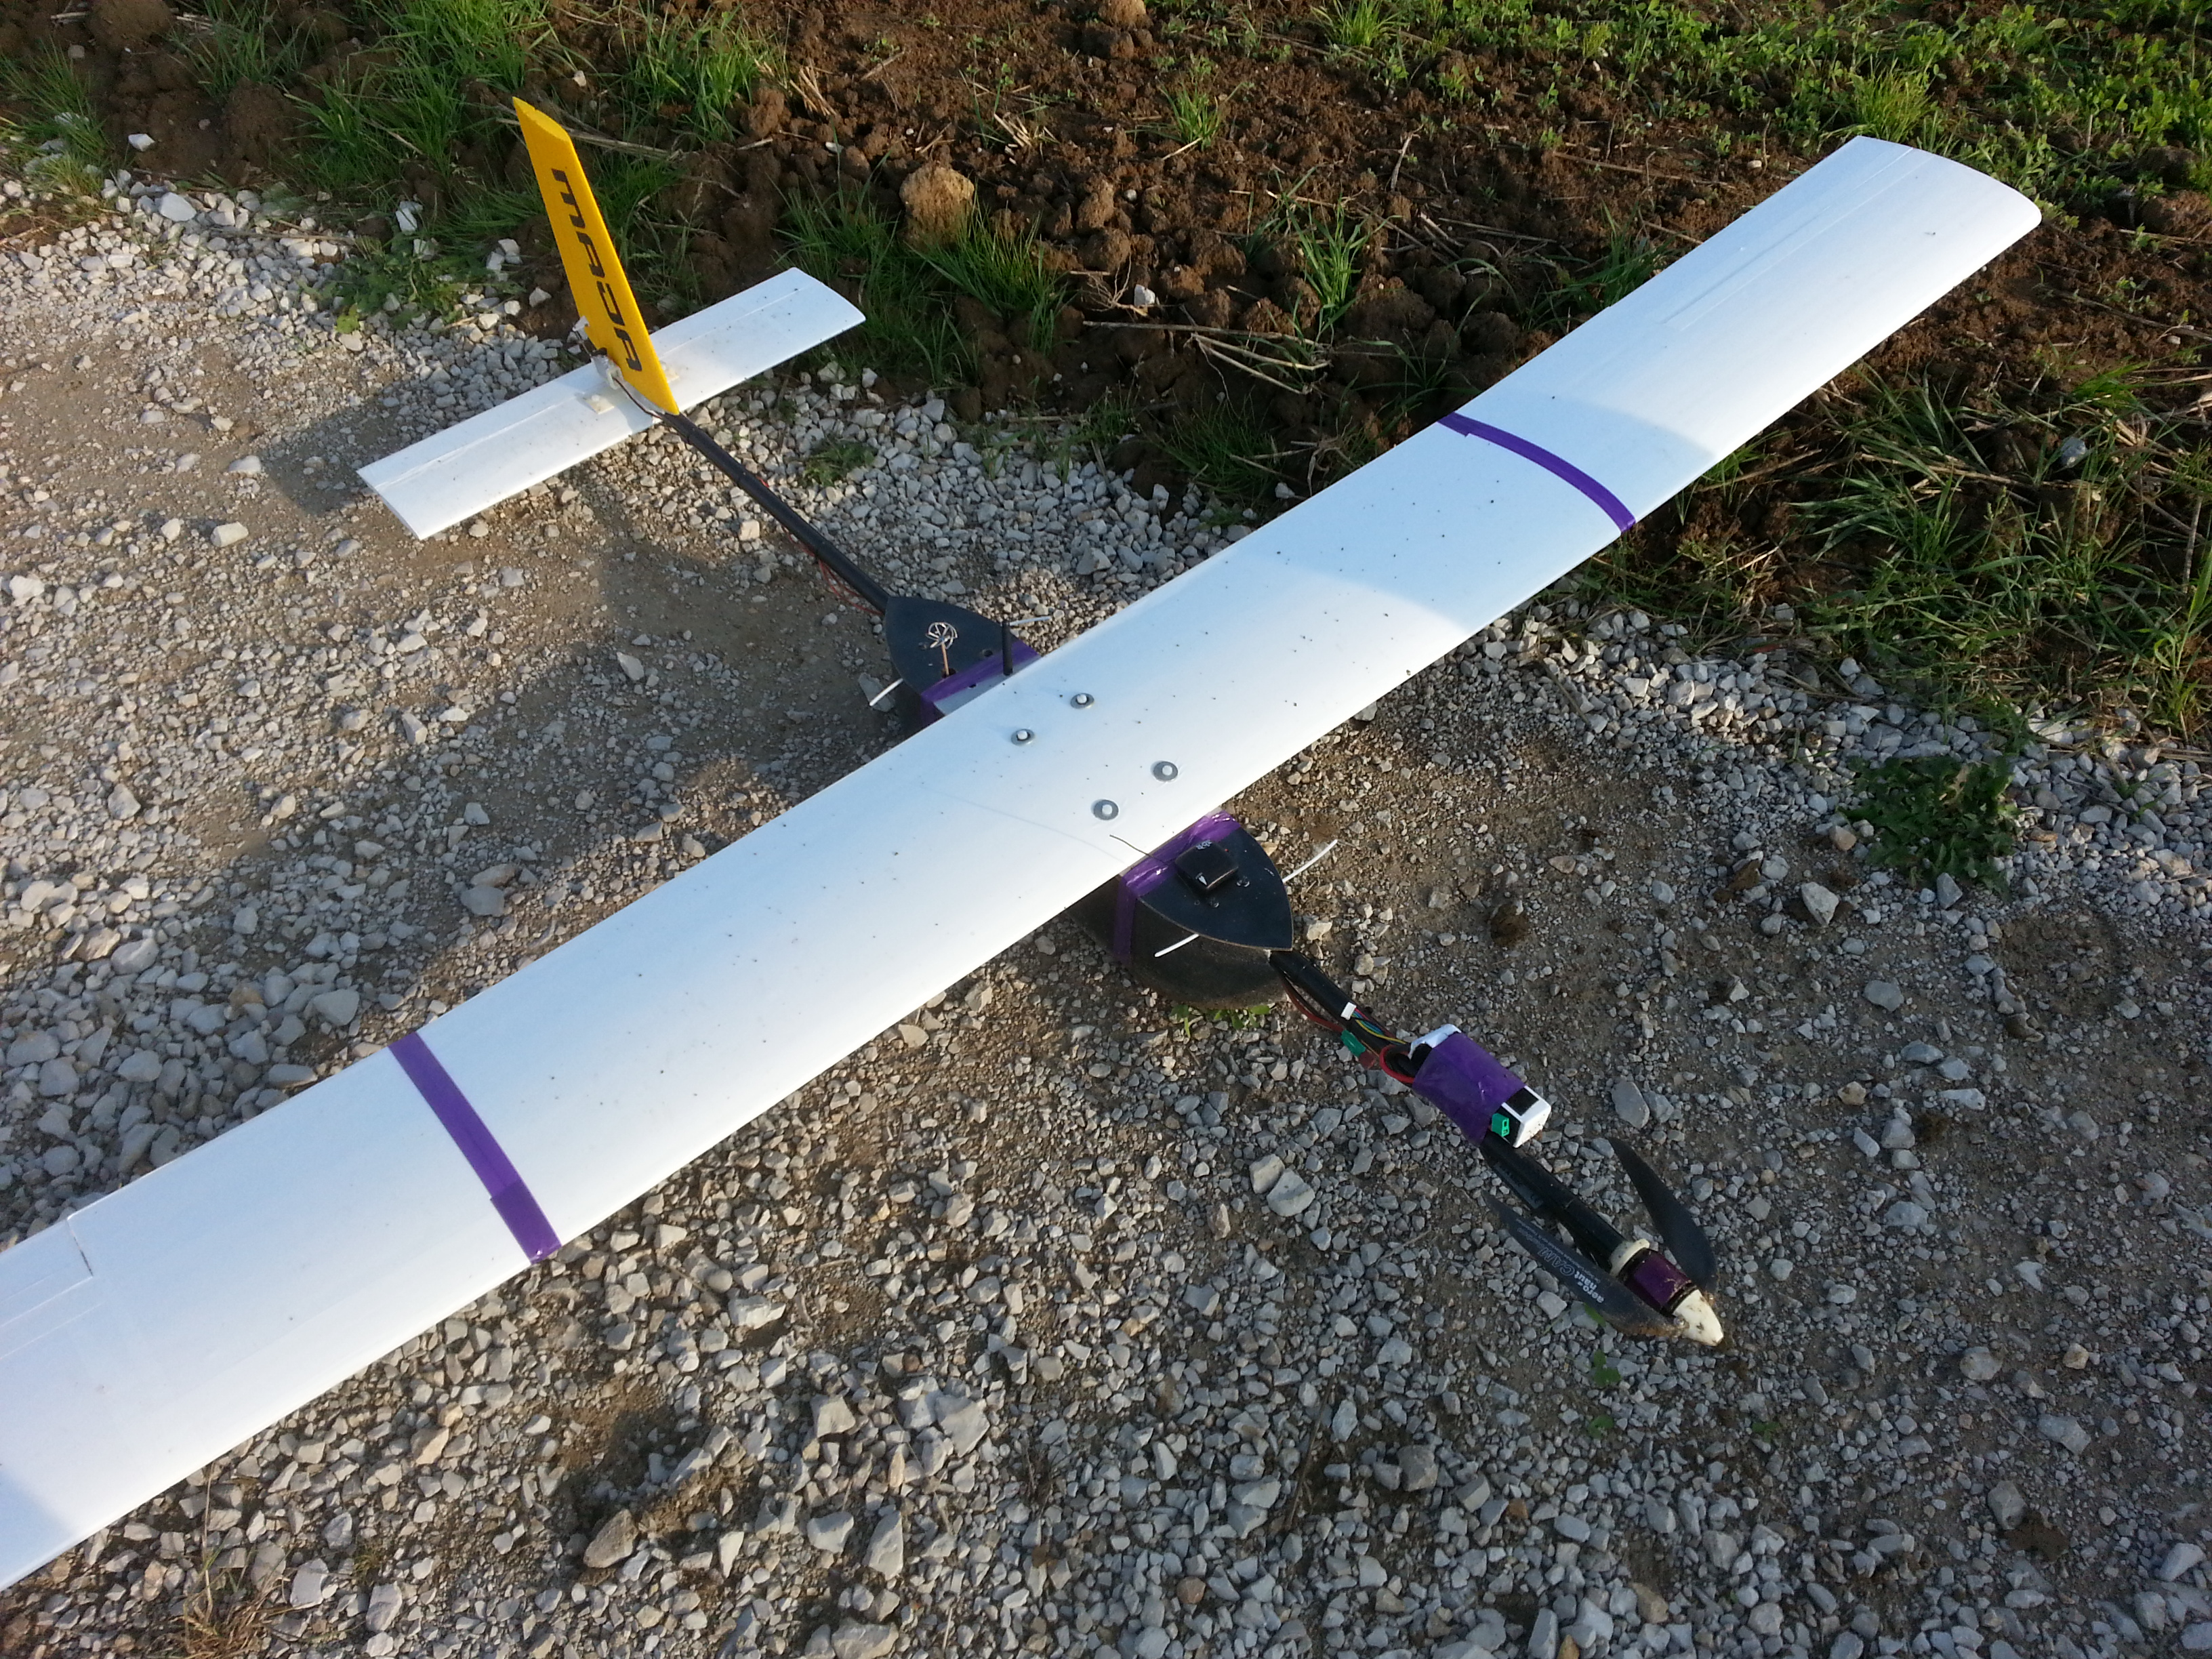
\includegraphics[width=0.9\textwidth]{bilder/Fotos/AUVSI-MAYA-Hybrid.jpg} 
\caption{Frühe Vorversuche für das AUVSI 2015 Flugzeug} 
\label{Frühe Vorversuche für das AUVSI 2015 Flugzeug}
\end{figure}

Daraus reiften das erste Konzept für einen selbst Konstruierten und Hergestellten Flieger. Die Flügel und Ruder waren in Klassischer Balsa beplankter Styroporbauweise ausgeführt die so bis heute im Einsatz ist. Erstmals war hier auch der Verfügbare Platz im Rumpfsegment an die Komponenten Angepasst. Während sich das neue Flugzeug an sich bewährte wurde der Rumpf als schlecht zu Handhaben und unzugänglich kritisiert.

\begin{figure}[H]
\centering
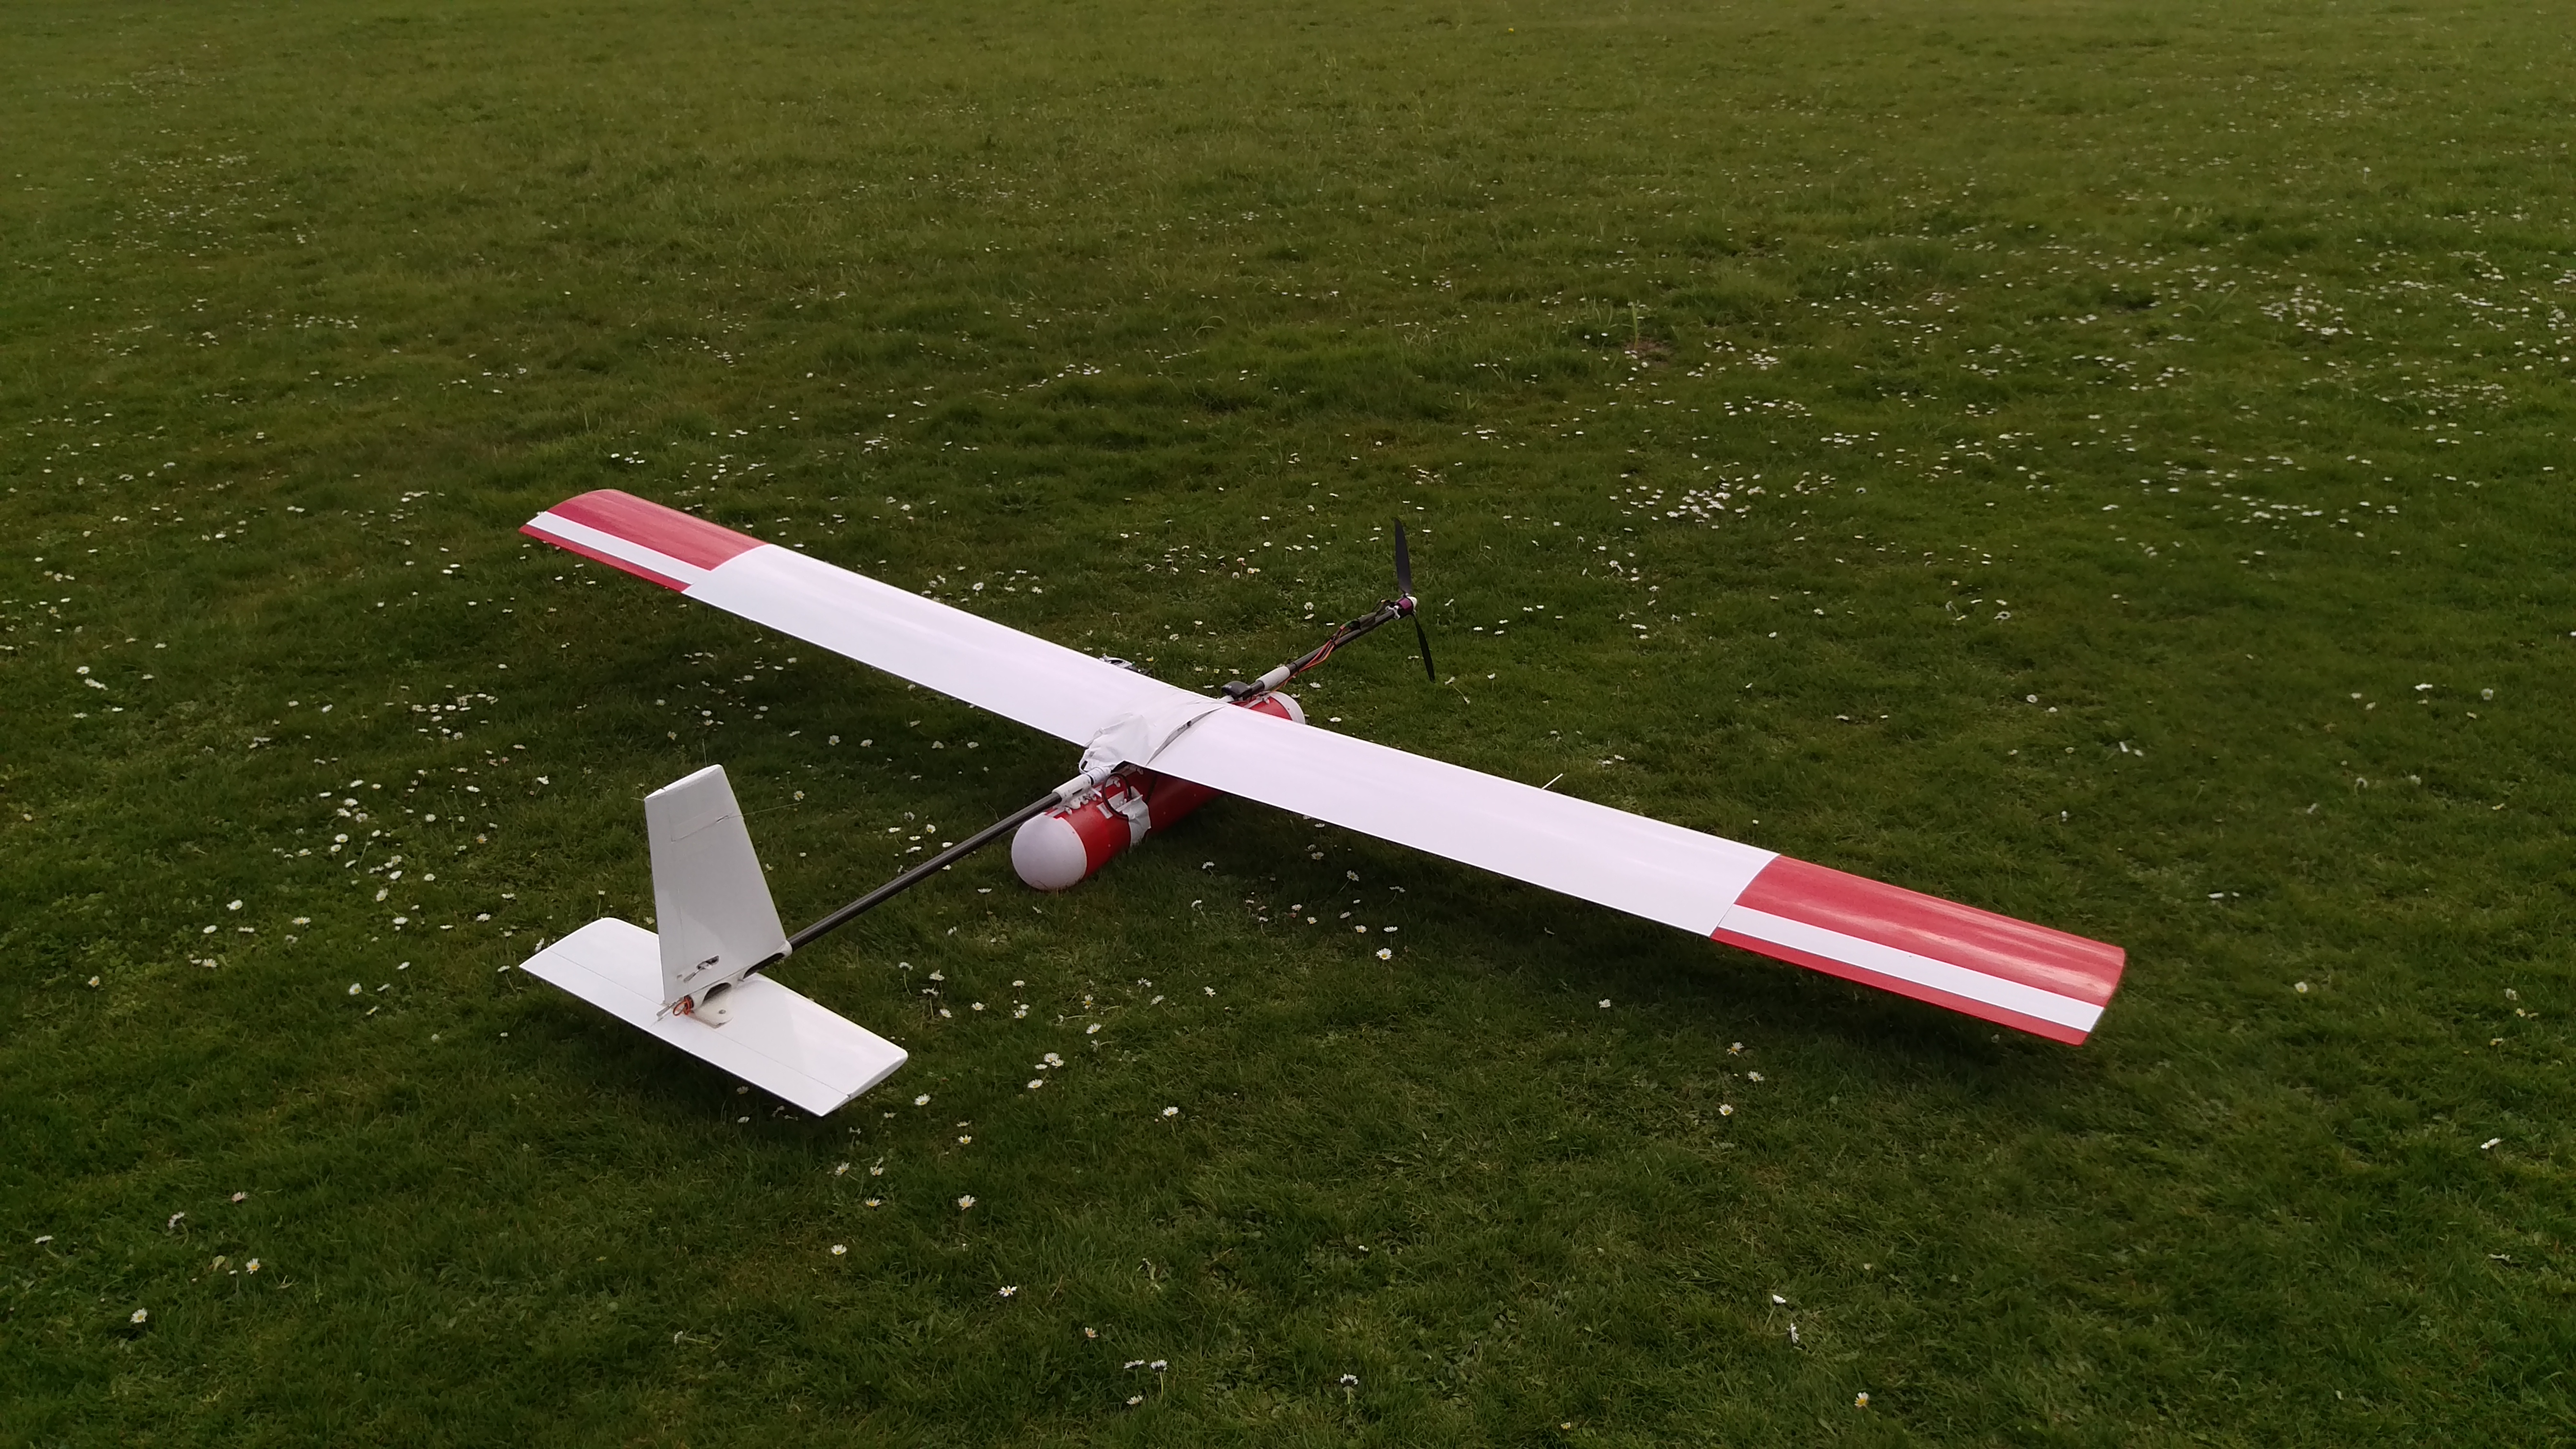
\includegraphics[width=0.9\textwidth]{bilder/Fotos/AUVSI_2015.jpg} 
\caption{Das AUVSI 2015 Modell in Einsatzzustand am Testflugplatz} 
\label{Das AUVSI 2015 Modell in Einsatzzustand am Testflugplatz}
\end{figure}

Damit entstand im Laufe der Arbeiten zur ersten eigenen Teilnahme am AUVSI Wettbewerb 2015 ein voll Modulares Hardware Konzept für Flügelkasten, Leitwerk, Leitwerksträger und Nutzlastrumpf.
Damit war eine gute Handhabung der einzelnen Sektionen bei Missionsvorbereitung und Modifikationen möglich. Integriert war hier auch die erste Generation einer eigenen Flugzeugbordelektronik für Leistungs und Signalpfade. Das auch über zahlreiche Testflüge gereifte Flugsystem konnte so auf dem Wettbewerb einen erfolgreichen siebten Platz erzielen.

\begin{figure}[H]
\centering
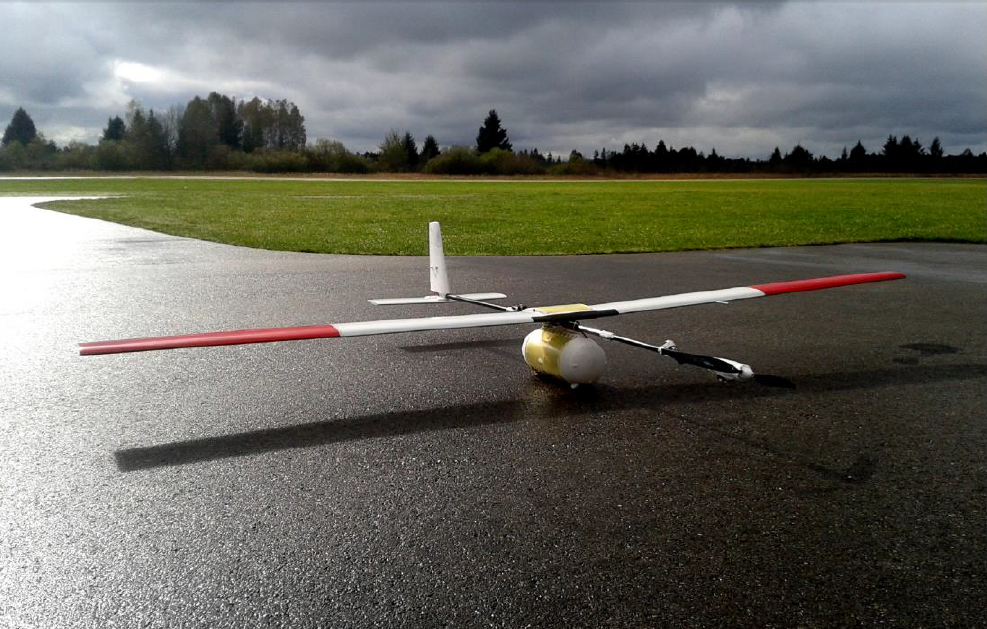
\includegraphics[width=0.9\textwidth]{bilder/Fotos/Ecuadorflieger_Koenigsdorf.png} 
\caption{Für die Fotomission in Ecuador modifizierter AUVSI 2015 Flieger in Königsdorf} 
\label{Für die Fotomission in Ecuador modifizierter AUVSI 2015 Flieger in Königsdorf}
\end{figure}

Im weiteren Verlauf des Jahres 2015 wurde das Forschungs Kooperationsprojekt mit der Fakultät für Geoinformatik in Angriff genommen. Die bewährte AUVSI 2015 Plattform wurde mit einem neuen Nutzlastrumpf nach dem Selben Modulprinzip ausgestatt der diesmal primär eine Hochauflösende Spiegelreflexkamara für Reihenbildaufnahmen trug. Es konnten zahlreiche routinierte Missionsflüge im Regenwald Ecuadors durchgeführt werden.

\begin{figure}[H]
\centering
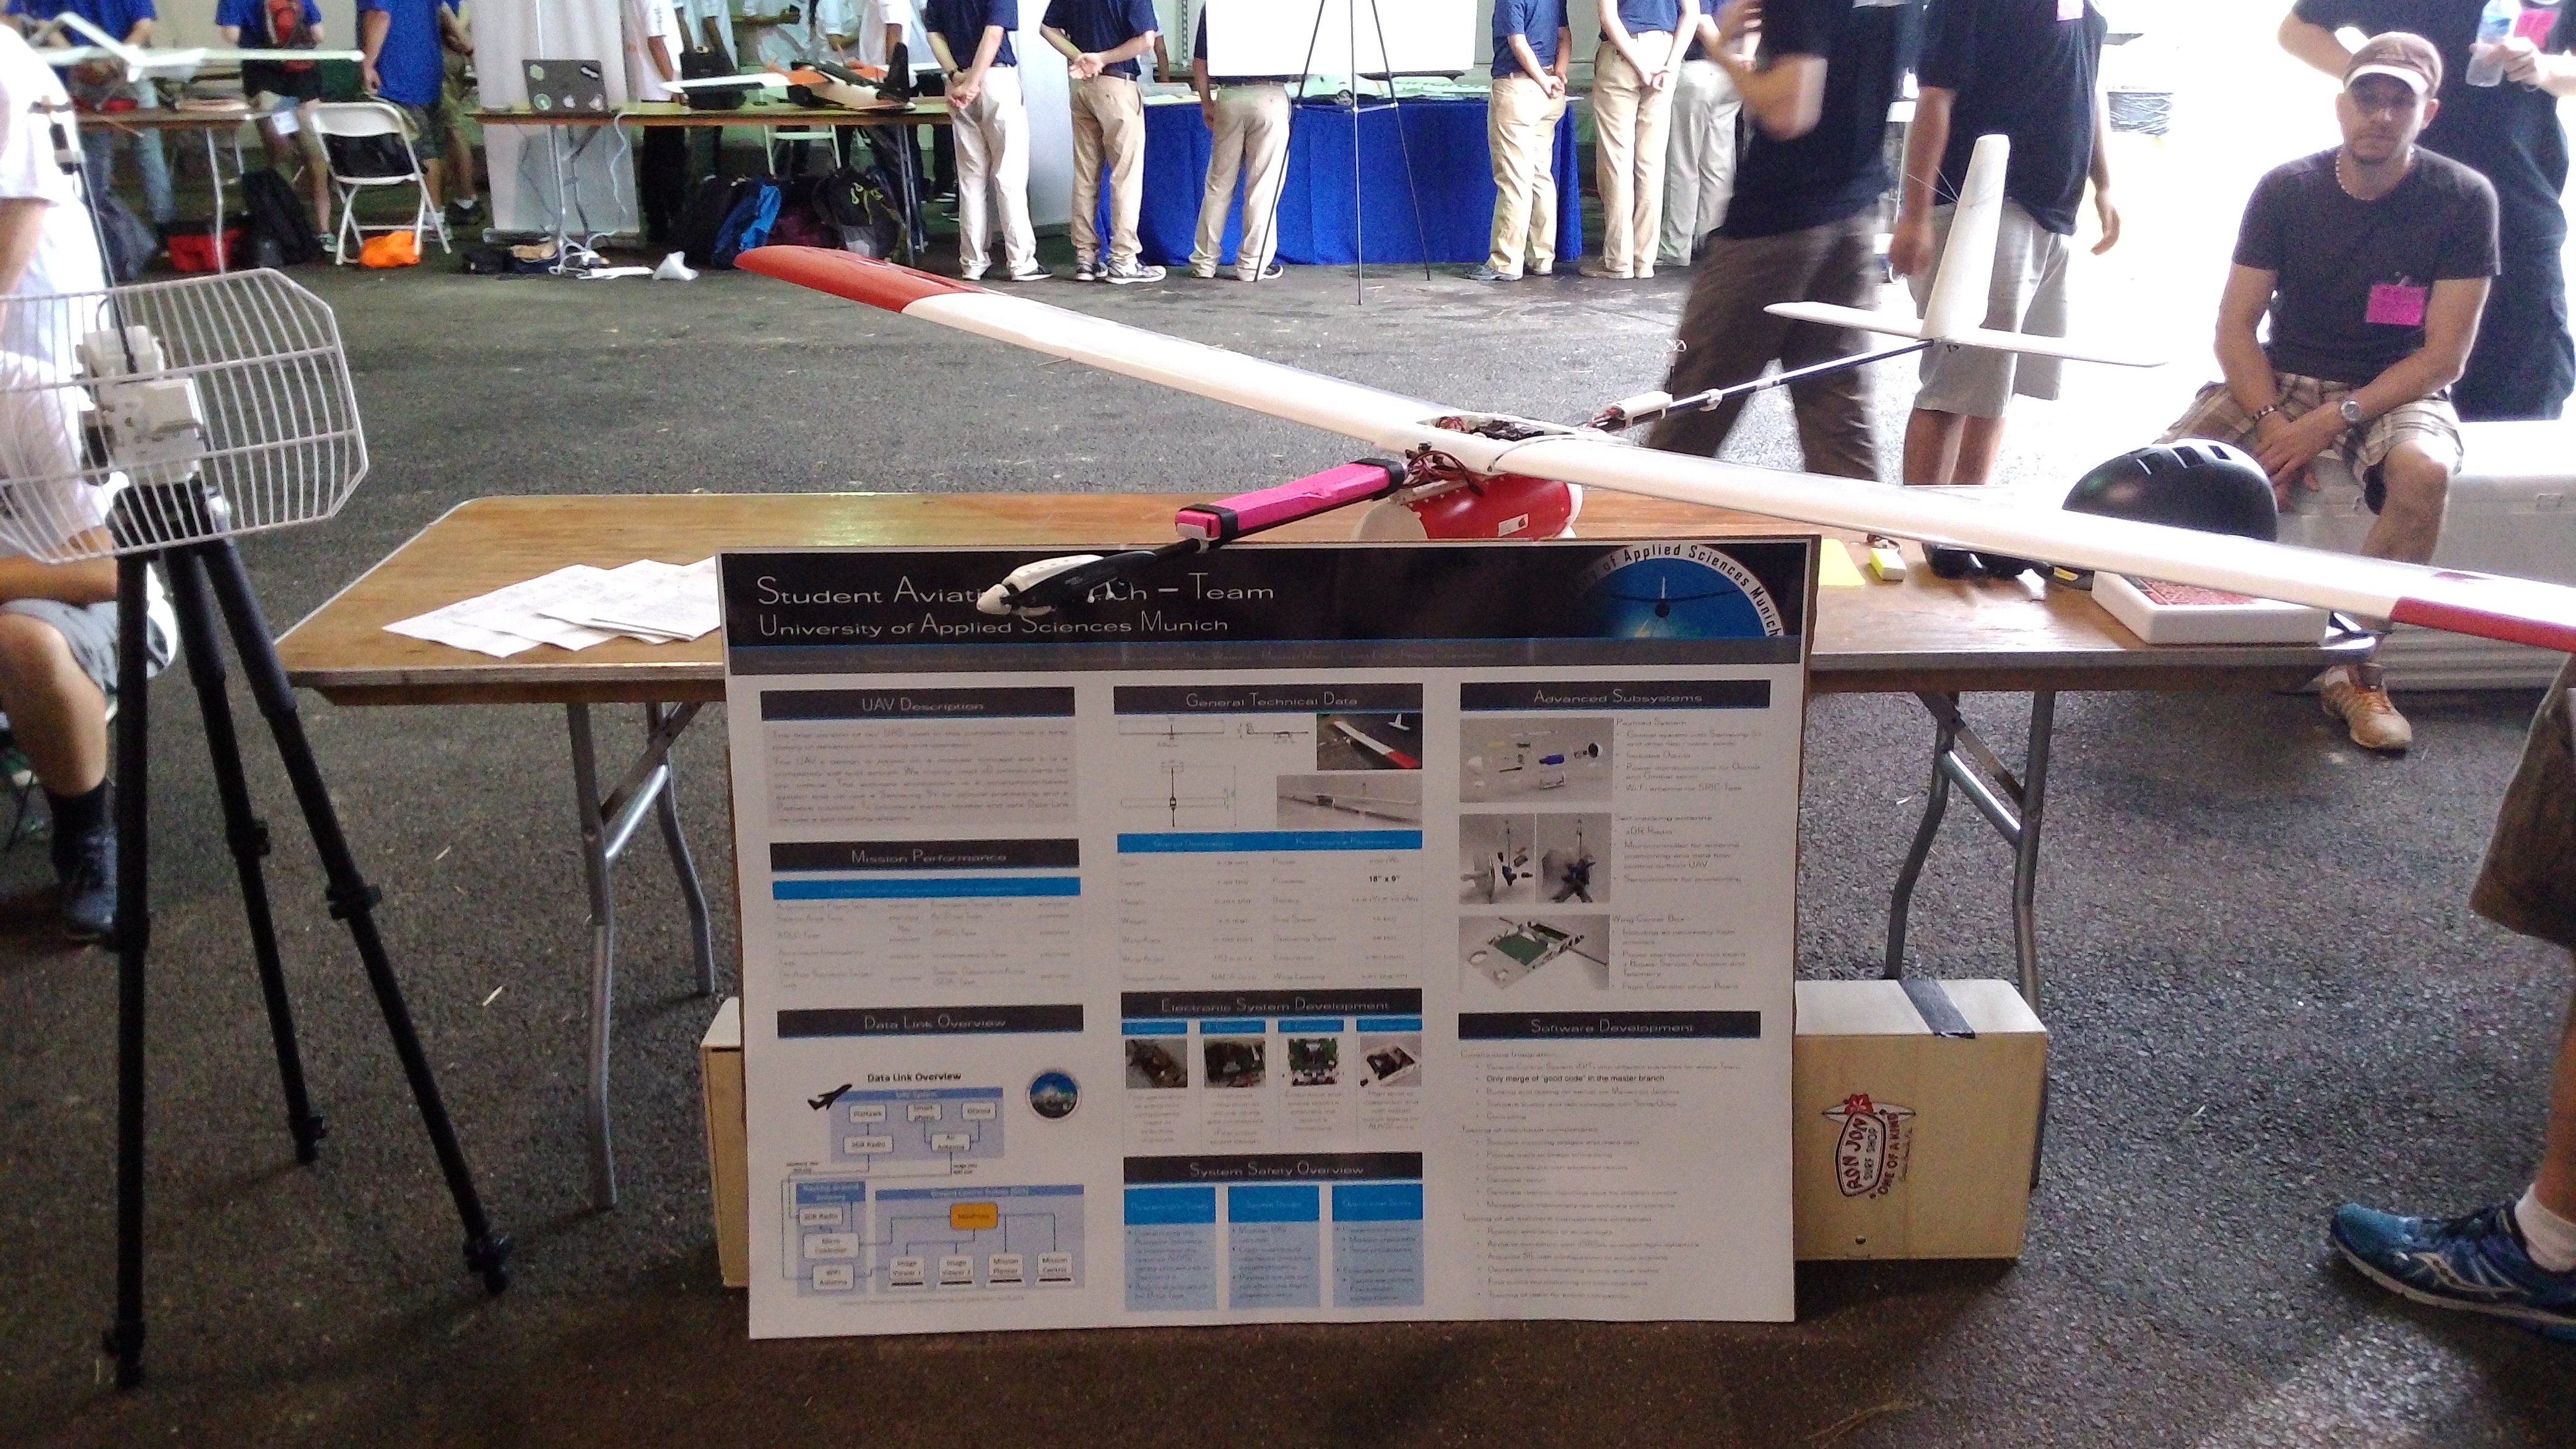
\includegraphics[width=0.9\textwidth]{bilder/Fotos/AUVSI_2016_Display.jpg} 
\caption{Der AUVSI 2016 Flieger beim Display auf dem Wettberwerb} 
\label{Der AUVSI 2016 Flieger beim Display auf dem Wettberwerb}
\end{figure}

Der AUVSI 2016 Flieger stellt eine konsequente Weiterentwicklung mit den Erfahrungen von AUVSI 2015 und der Ecuadormission dar. Erstmals wurden die Batterisysteme in die Flügel verlegt um Platz und mechanische Belastungen zu sparen. Eine neue Generation der Bordelektronik ermöglichte die Fremdversorgung der Missionsklaren Fliegers beim warten auf den Start. Die geänderten Anforderungen an Kamerasysteme und Bordcomputer konnten in einen deutlich Verkleinerten Rumpf umgesetzt werden. 